\documentclass{beamer}
\mode<presentation>
\usetheme{CambridgeUS}
\usepackage[russian]{babel}
\usepackage[utf8]{inputenc}
\usepackage[T2A]{fontenc}
\usepackage{sansmathaccent}

\usepackage{verbatim}
\usepackage{alltt}

\pdfmapfile{+sansmathaccent.map}
\title[Artifical Intelligence]{Обработка текста на естественном языке}
\author{Наумов Д.А., доц. каф. КТ}
\date[26.02.2020] {Экспертные системы и искусственный интеллект, 2019}

\begin{document}

%ТИТУЛЬНЫЙ СЛАЙД
\begin{frame}
  \titlepage
\end{frame}
  
%СОДЕРЖАНИЕ ЛЕКЦИИ
\begin{frame}
  \frametitle{Содержание лекции}
  \tableofcontents  
\end{frame}

\section{Строковые данные}

\begin{frame}{Введение}
Типы признаков, которые могут представлять свойства данных:
\begin{itemize}
\item непрерывные признаки, описывающие количество;
\item категориальные признаки, которые являются элементами фиксированного списка;
\item текст.
\end{itemize}
Пример: 
\begin{itemize}
\item классифицировать сообщения электронной почты на спам и действительно нужные письма;
\item узнать мнение какого-то политика об иммиграции из текстов его выступлений или твитов;
\item выяснить, является ли сообщение жалобой или запросом, проанализировав тему и содержание сообщения.
\end{itemize}
\end{frame}

\begin{frame}{Введение}
Строковые данные:
\begin{itemize}
\item категориальные данные;
\item неструктурированные строки, которые по смыслу можно сгруппировать в категории;
\item структурированные строки;
\item текстовые данные.
\end{itemize}
\begin{block}{Категориальные данные (categorical data)}
представляют собой данные, которые берутся из фиксированного списка. 
\end{block}
\begin{block}{Неструктурированне строки}
ответы, записанные в текстовом поле, которые по смыслу можно сгруппировать в категории.
\end{block}
\end{frame}

\begin{frame}{Введение}
\begin{block}{Структурированные строки}
строковые значения, введенные вручную, не соответствующие фиксированным категориям, но при этом все же имеющие некоторую базовую структуру, например, адреса, названия мест, имена и фамилии людей, даты, номера телефонов и другие идентификаторы.
\end{block}
\begin{block}{Текстовые данные}
оторые состоят из фраз или предложений. 
\end{block}
Пример:
\begin{itemize}
\item твиты, логи чата;
\item отзывы о гостинице;
\item собрание сочинений Шекспира;
\item содержание Википедии.
\end{itemize}
\end{frame}

\section{Обработка естественного языка}

\begin{frame}{NLP}
Обработка естественного языка (Natural Language Processing, NLP) - важная частью современных систем. 
\begin{block}{Цель NLP}
разработка алгоритмов, которые позволяли бы компьютерам распознавать свободный текст и понимать живую речь. 
\end{block}
Области применения:
\begin{itemize}
\item поисковые системы;
\item речевые интерфейсы;
\item процессоры документов.
\end{itemize}
Применения подходов на основе машинного обучения: 
\begin{itemize}
\item сбор огромных массивов текста (для понимания контекста);
\item обучение алгоритма для выполнения различных задач (категоризация текста, сентимент-анализ,  тематическое моделирование).
\end{itemize}
\end{frame}

\begin{frame}{Пример: анализ тональности киноотзывов}
Воспользуемся набором данных, который содержит киноотзывы, оставленные на сайте IMDВ.
\begin{itemize}
\item собранны исследователем Стэнфордского университета Эндрю Маасом;
\item набор данных доступен по ссылке http://ai.stanford.edu/~amaas/data/sentiment/;
\item набор содержит тексты отзывов, а также метки, которые указывают тональность отзыва (<<положительный>> или <<отрицательный>>).
\end{itemize}
\begin{figure}[h]
\centering
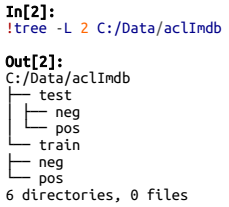
\includegraphics[scale=0.5]{images/lec09-pic01.png}
\end{figure}
\end{frame}

\begin{frame}{Пример: анализ тональности киноотзывов}
В библиотеке scikit-learn есть вспомогательная функция load\_files. Она позволяет загрузить файлы,
для хранения которых используется такая структура папок, где каждая вложенная папка соответствует определенной метке. Применим функцию load\_files к обучающим данным:
\begin{figure}[h]
\centering
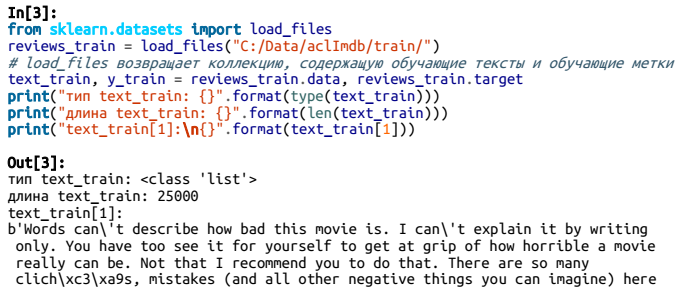
\includegraphics[scale=0.6]{images/lec09-pic02.png}
\end{figure}
\end{frame}

\begin{frame}{Пример: анализ тональности киноотзывов}
\begin{itemize}
\item text\_train - список длиной 25000, в котором каждый элемент представляет собой строку, содержащую отзыв.
\item отзыв содержит разрывы строк HTML (br). Хотя эти разрывы вряд ли сильно повлияют на модель машинного обучения, лучше выполнить очистку данных и удалить символы форматирования перед тем, как начать работу.
\end{itemize}
\begin{figure}[h]
\centering
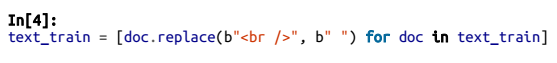
\includegraphics[scale=0.75]{images/lec09-pic03.png}
\end{figure}
\end{frame}

\begin{frame}{Пример: анализ тональности киноотзывов}
Набор данных был собран таким образом, чтобы положительный и отрицательный классы были сбалансированы.
\begin{figure}[h]
\centering
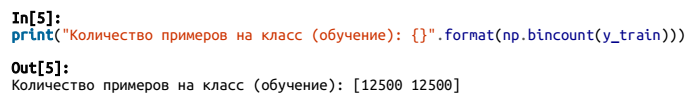
\includegraphics[scale=0.6]{images/lec09-pic04.png}
\end{figure}
Аналогичным образом загружаем тестовые данные:
\begin{figure}[h]
\centering
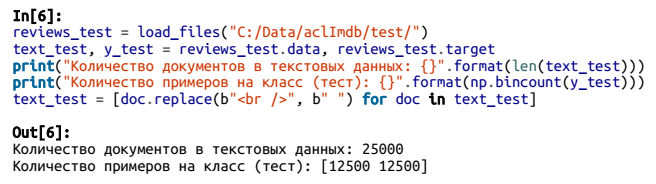
\includegraphics[scale=0.6]{images/lec09-pic05.png}
\end{figure}
\end{frame}

\begin{frame}{Пример: анализ тональности киноотзывов}
\begin{block}{Постановка задачи}
каждому отзыву нам нужно присвоить метку <<положительный>> или <<отрицательный>> на основе текста отзыва.
\end{block}
\begin{itemize}
\item это стандартная задача бинарной классификации, однако текстовые данные представлены в формате, который модель машинного обучения не умеет обрабатывать. 
\item необходимо преобразовать строковое представление текста в числовое представление, к которому можно применить алгоритмы машинного обучения.
\end{itemize}
\end{frame}

\section{Мешок слов}

\begin{frame}
С точки зрения анализа текста набор данных часто называют \textbf{корпусом} (corpus) и каждая точка данных, представленная в виде отдельного текста, называется \textbf{документом} (document). 
\begin{block}{Мешок слов, bag-ofwords}
представление, в котором удалена структура исходного текста (главы, параграфы, предложения, форматирование) и подсчитана частота встречаемости каждого слова в каждом документе корпуса.
\end{block}
Три этапа получения мешка слов:
\begin{enumerate}
\item \textbf{Токенизация} (tokenization). Разбиваем каждый документ на слова, которые встречаются в нем (токены), например, с помощью пробелов и знаков пунктуации.
\item \textbf{Построение словаря} (vocabulary building). Собираем словарь всех слов, которые появляются в любом из документов, и пронумеровываем их (например, в алфавитном порядке).
\item \textbf{Создание разреженной матрицы} (sparse matrix encoding). Для каждого документа подсчитываем, как часто каждое из слов, занесенное в словарь, встречается в документе.
\end{enumerate}
\end{frame}

\begin{frame}{Обработка <<мешок слов>>}
\begin{figure}[h]
\centering
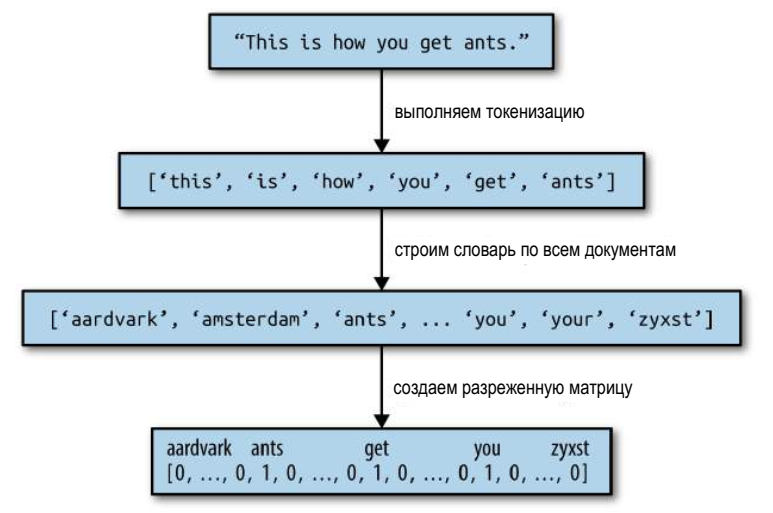
\includegraphics[scale=0.5]{images/lec09-pic06.png}
\end{figure}
\end{frame}

\begin{frame}{Пример: <<мешок слов>> для синтетического набора данных}
Модель «мешка слов» реализована в классе CountVectorizer, который выполняет соответствующее преобразование. 
\begin{figure}[h]
\centering
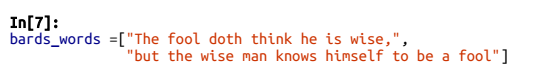
\includegraphics[scale=0.7]{images/lec09-pic07.png}
\end{figure}
Импортируем класс CountVectorizer, создам экземпляр класса и подгоняем модель к нашим синтетическим данным следующим образом:
\begin{figure}[h]
\centering
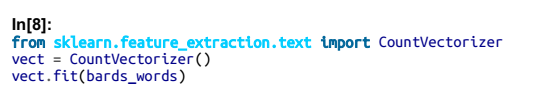
\includegraphics[scale=0.7]{images/lec09-pic08.png}
\end{figure}
\end{frame}

\begin{frame}
Процесс подгонки CountVectorizer включает в себя токенизацию обучающих данных и построение словаря, к которому мы можем получить доступ с помощью атрибута vocabulary\_: 
\begin{figure}[h]
\centering
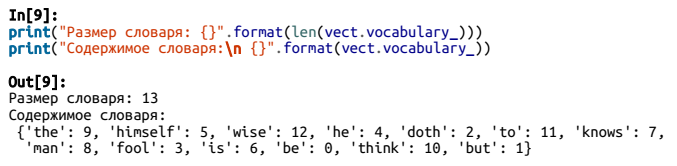
\includegraphics[scale=0.6]{images/lec09-pic09.png}
\end{figure}
Словарь состоит из 13 слов, начинается со слова «be» и заканчивается словом «wise». Чтобы получить «мешок слов», вызываем метод transform:
\begin{figure}[h]
\centering
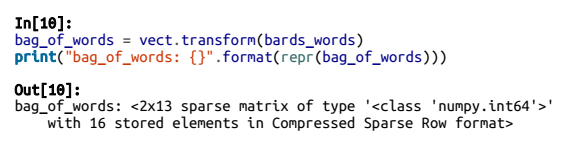
\includegraphics[scale=0.6]{images/lec09-pic10.png}
\end{figure}
\end{frame}

\begin{frame}{Пример: <<мешок слов>> для синтетического набора данных}
Представление «мешок слов» записывается в разреженной матрице SciPy, которая хранит только ненулевые элементы. Чтобы взглянуть на фактическое содержимое разреженной матрицы, мы можем
преобразовать ее в «плотный» массив NumPy: 
\begin{figure}[h]
\centering
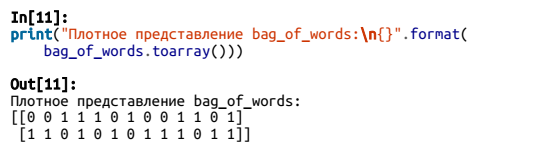
\includegraphics[scale=0.75]{images/lec09-pic11.png}
\end{figure}
\end{frame}

\begin{frame}{Пример: <<мешок слов>> для киноотзывов}
Обработаем обучающие и тестовые данные, сформированные на основе отзывов IMDb, в виде списков строк (text\_train и text\_test): 
\begin{figure}[h]
\centering
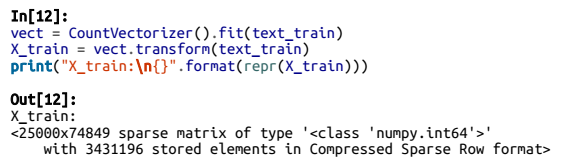
\includegraphics[scale=0.75]{images/lec09-pic12.png}
\end{figure}
Матрица X\_train соответствует обучающим данным, представленным в виде «мешка слов». Она имеет форму 25000 x 74849, указывая на то, что словарь включает 74849 элементов в разреженной матрицы SciPy.
\end{frame}

\begin{frame}
Еще один способ получить доступ к словарю – это использование метода get\_feature\_name. Он возвращает удобный список, в котором каждый элемент соответствует одному признаку: 
\begin{figure}[h]
\centering
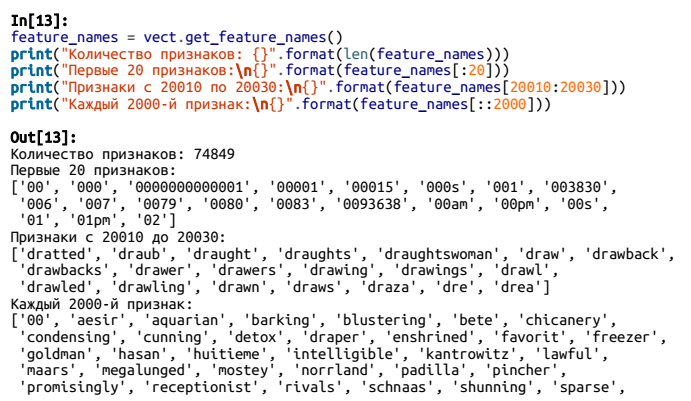
\includegraphics[scale=0.5]{images/lec09-pic13.png}
\end{figure}
Проблемы: числа, выделение значимой информации, обработка форм слов. 
\end{frame}

\section{Построение модели}

\begin{frame}
Как правило, для подобных высокоразмерных разреженных данных лучше всего работают линейные модели типа LogisticRegression. 

Измерим качество модели, построив классификатор: 
\begin{figure}[h]
\centering
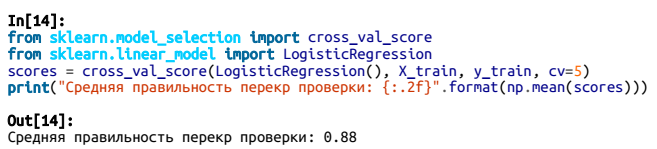
\includegraphics[scale=0.75]{images/lec09-pic14.png}
\end{figure}
Среднее значение правильности перекрестной проверки - 88\%, что указывает на приемлемое качество модели для задачи сбалансированной бинарной классификации.
\end{frame}

\begin{frame}
Логистическая регрессия имеет параметр регуляризации C, который мы можем настроить с помощью перекрестной проверки: 
\begin{figure}[h]
\centering
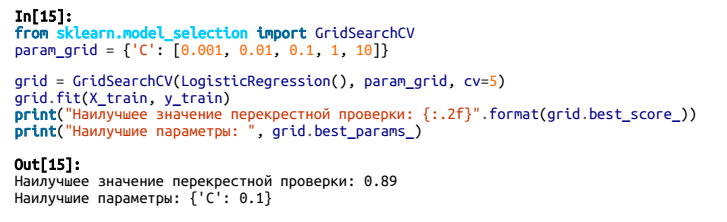
\includegraphics[scale=0.75]{images/lec09-pic15.png}
\end{figure}
\end{frame}

\begin{frame}
Будем использовать только те токены, которые встречаются по крайней мере в двух документах (или по крайней мере в пяти документах и т.д.), задавания параметр min\_df: 
\begin{figure}[h]
\centering
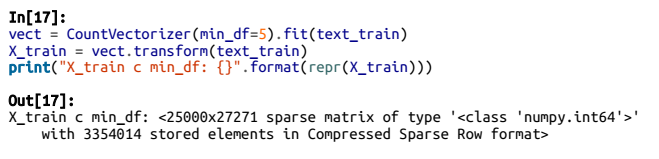
\includegraphics[scale=0.75]{images/lec09-pic16.png}
\end{figure}
\end{frame}

\begin{frame}
Задав min\_df=5, мы уменьшаем количество признаков до 27271, и если сравнить этот результат с предыдущим выводом, теперь мы используем лишь треть исходных признаков: 
\begin{figure}[h]
\centering
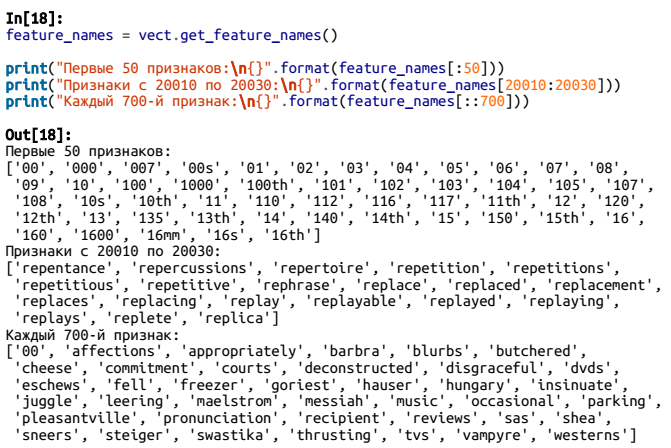
\includegraphics[scale=0.5]{images/lec09-pic17.png}
\end{figure}
\end{frame}

\begin{frame}
Четко видно, что намного реже стали встречаться числа и, похоже, что
исчезли некоторые странные или неправильно написанные слова. 

Оценим качество нашей модели, вновь выполнив решатчатый поиск: 
\begin{figure}[h]
\centering
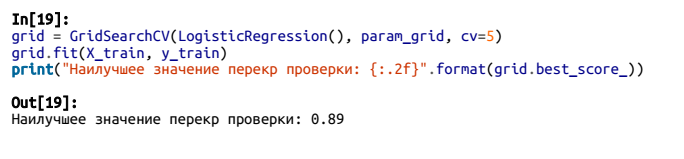
\includegraphics[scale=0.6]{images/lec09-pic18.png}
\end{figure}
Наилучшее значение правильности, полученное в ходе перекрестной проверки, по-прежнему равно 89\%. Мы не смогли улучшить качество нашей модели, однако сокращение количества признаков ускорит предварительную обработку.
\end{frame}

\section{Стоп-слова}

\begin{frame}{Стоп-слова}
Мы можем избавиться от неинформативных слов:
\begin{itemize}
\item использование списка стоп-слов (на основе соответствующего языка);
\item удаление слов, которые встречаются слишком часто.
\end{itemize}
Библиотека scikit-learn предлагает встроенный список английских стоп-слов, реализованный в модуле feature\_extraction.text: 
\begin{figure}[h]
\centering
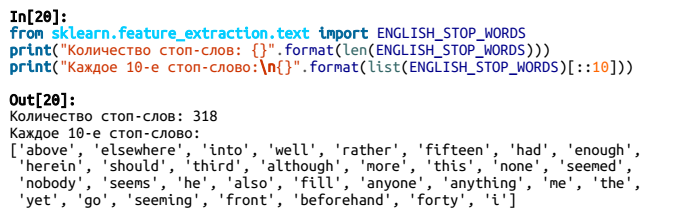
\includegraphics[scale=0.6]{images/lec09-pic19.png}
\end{figure}
\end{frame}

\begin{frame}{Стоп-слова}
Удаление стоп-слов с помощью списка может уменьшить количество признаков лишь ровно на то количество, которое есть в списке (318), но, возможно, это позволит улучшить качество
модели:
\begin{figure}[h]
\centering
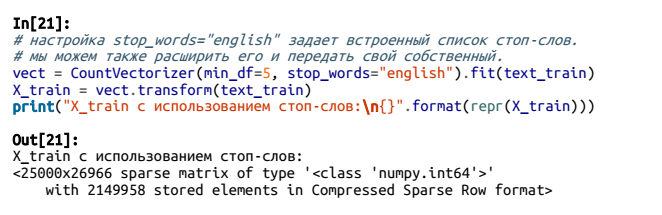
\includegraphics[scale=0.6]{images/lec09-pic20.png}
\end{figure}
Теперь у нас стало на 305 признаков меньше (количество признаков уменьшилось с 27271 до 26966). Это означает, что большинство стопслов (но не все) встретились в корпусе документов.
\end{frame}

\begin{frame}{Стоп-слова}
Снова запустим решетчатый поиск:
\begin{figure}[h]
\centering
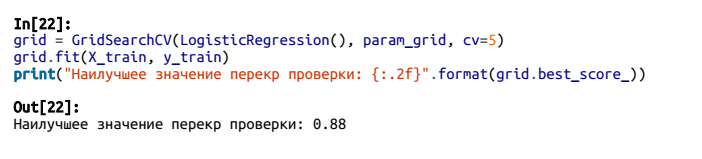
\includegraphics[scale=0.6]{images/lec09-pic21.png}
\end{figure}
\begin{itemize}
\item качество модели чуть снизилось;
\item исключили 305 признаков из более чем 27000;
\item использование списка стоп-слов в данном случае бесполезно;
\item фиксированные списки могут быть полезны при работе с небольшими наборами данных;
\item можно попробовать другой подход, задав опцию max\_df для CountVectorizer.
\end{itemize}
\end{frame}

\section{Масштабирование данных при помощи tf-idf}

\begin{frame}{Масштабирование данных при помощи tf-idf}
\begin{block}{Частота термина-обратная частота документа (term frequency-inverse document frequency, tf-idf)}
идея заключается в том, чтобы присвоить большой вес термину, который часто встречается в конкретном документе, но при этом редко встречается в остальных документах корпуса.
\end{block}
\begin{figure}[h]
\centering
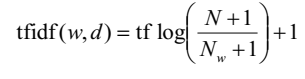
\includegraphics[scale=0.5]{images/lec09-pic22.png}
\end{figure}
\begin{itemize}
\item N – количество документов в обучающем наборе, 
\item Nw – количество документов обучающего набора, в которых встретилось слово w, 
\item tf (частота термина) – это частота встречаемости термина в запрашиваемом документе d (документе, который вы хотите преобразовать).
\end{itemize}
\end{frame}

\begin{frame}{Масштабирование данных при помощи tf-idf}
В библиотеке scikit-learn метод tf-idf реализован в двух классах: 
\begin{itemize}
\item TfidfTransformer, который принимает на вход разреженную матрицу, полученную с помощью CountVectorizer и преобразует ее; 
\item TfidfVectorizer, который принимает на вход текстовые данные и выполняет как выделение признаков «мешок слов», так и преобразование tf-idf. 
\end{itemize}
Воспользуемся конвейером, чтобы убедиться в достоверности результатов нашего решетчатого поиска:
\begin{figure}[h]
\centering
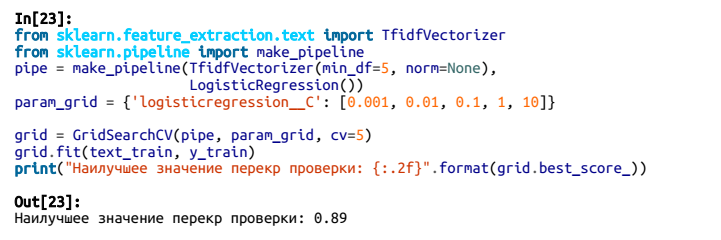
\includegraphics[scale=0.5]{images/lec09-pic23.png}
\end{figure}
\end{frame}

\begin{frame}{Масштабирование данных при помощи tf-idf}
Мы можем выяснить, какие слова в результате преобразования tf-idf стали наиболее важными.
\begin{figure}[h]
\centering
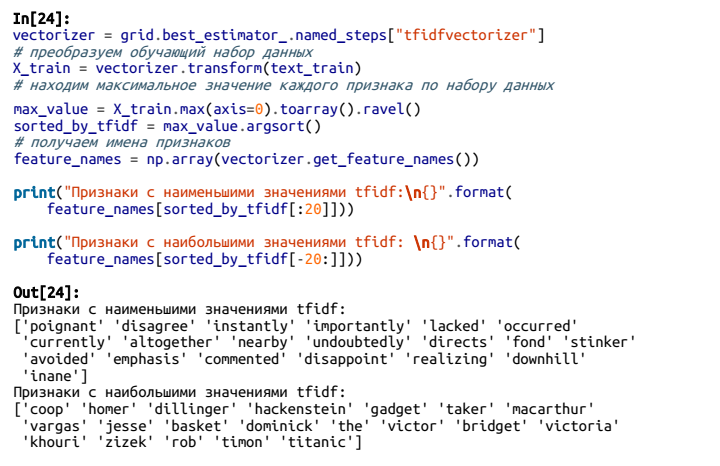
\includegraphics[scale=0.75]{images/lec09-pic24.png}
\end{figure}
\end{frame}

\begin{frame}{Масштабирование данных при помощи tf-idf}
\begin{itemize}
\item признаки с низкими значениями tf-idf – это признаки, которые либо встречаются во многих документах, либо используются редко и только в очень длинных документах. 
\item многие признаки с высокими значениями tf-idf на самом деле соответствуют названиям некоторых шоу или фильмов. Эти термины встречаются лишь в отзывах, посвященным конкретному шоу или франшизе, но при этом онивстречаются в данных отзывах очень часто ("smallville" и "doodlebops").
\end{itemize}
\end{frame}

\begin{frame}
Мы можем найти слова, которые имеют низкое значение обратной частоты документа (атрибут idf\_):
\begin{figure}[h]
\centering
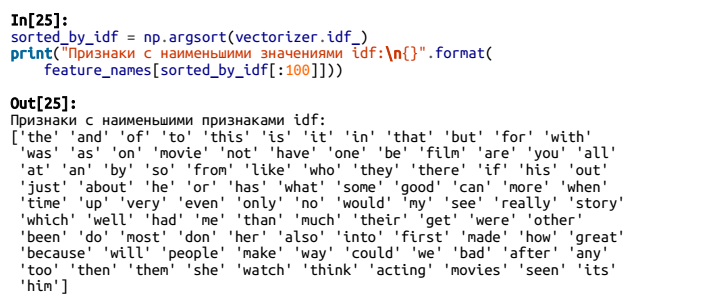
\includegraphics[scale=0.75]{images/lec09-pic25.png}
\end{figure}
\begin{itemize}
\item слова с низкими значениями idf стали английские стоп-слова типа "the" и "no";
\item некоторые характерны для киноотзывов: "movie", "film", "time", "story" и так далее. 
\item соответствии с метрикой tf-idf слова "good", "great" и "bad" также были отнесены к самым часто встречающимся и потому «самым нерелевантным» словам, хотя можно было бы ожидать, что они будут иметь очень важное значение для анализа тональности.
\end{itemize}
\end{frame}

\begin{frame}{Исследование коэффициентов модели}
Рассмотрим коэффициенты, получившие максимальные значения и их слова. 
\begin{figure}[h]
\centering
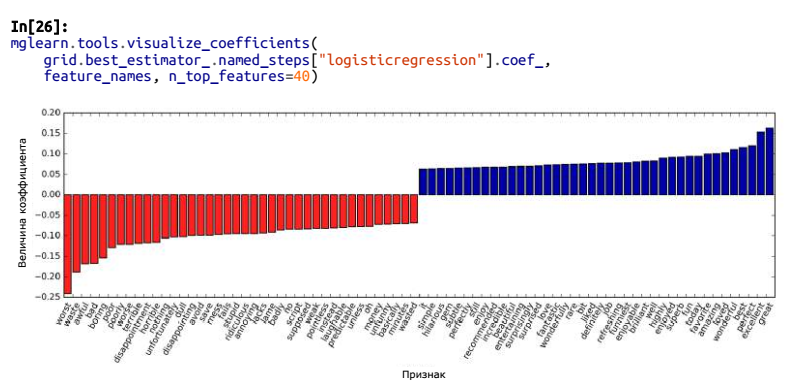
\includegraphics[scale=0.5]{images/lec09-pic26.png}
\end{figure}
Cледующая гистограмма показывает 25 наибольших и 25 наименьших коэффициентов модели логистической регрессии, каждый столбик соответствует величине коэффициента.
\end{frame}

\section{n-граммы}

\begin{frame}{Модель <<мешка слов>> для n-грамм}
Один из главных недостатков представления «мешок слов»: полное игнорировании порядка слов. Две строки   
\begin{itemize}
\item «it’s bad, not good at all» 
\item «it’s good, not bad at all» 
\end{itemize}
будут иметь одинаковое представление, хотя противоположны по смыслу.
\begin{block}{n-грамма}
последовательность токенов
\end{block}
\begin{itemize}
\item пары токенов - биграммами (bigrams);
\item тройки токенов - триграммы (trigrams);
\item последовательности из n токенов - n-граммы (n-grams). 
\end{itemize}
\end{frame}

\begin{frame}{Модель <<мешка слов>> для n-грамм}
\begin{itemize}
\item Мы можем изменить диапазон токенов, которые рассматриваются в качестве признаков, изменив
параметр ngram\_range для CountVectorizer или TfidfVectorizer.
\item Параметр ngram\_range задает нижнюю и верхнюю границы диапазона nзначений для различных извлекаемых n-грамм. 
\end{itemize}
\begin{figure}[h]
\centering
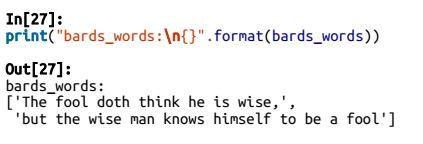
\includegraphics[scale=0.75]{images/lec09-pic27.png}
\end{figure}
\end{frame}

\begin{frame}{Модель <<мешка слов>> для n-грамм}
По умолчанию для каждой последовательности токенов с min\_n=1 и max\_n=1 (одиночные токены еще называются юниграммами или unigramms) CountVectorizer или TfidfVectorizer создает один признак:
\begin{figure}[h]
\centering
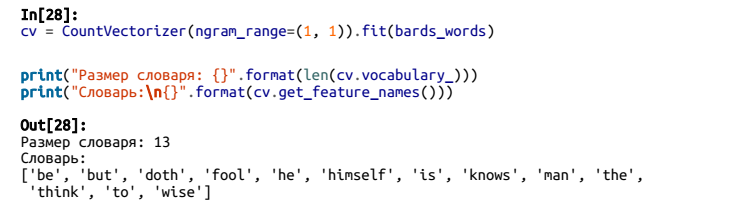
\includegraphics[scale=0.75]{images/lec09-pic28.png}
\end{figure}
\end{frame}

\begin{frame}{Модель <<мешка слов>> для n-грамм}
Чтобы посмотреть только биграммы, то есть последовательности из двух токенов, следующих друг за другом, мы можем задать ngram\_range равным (2, 2):
\begin{figure}[h]
\centering
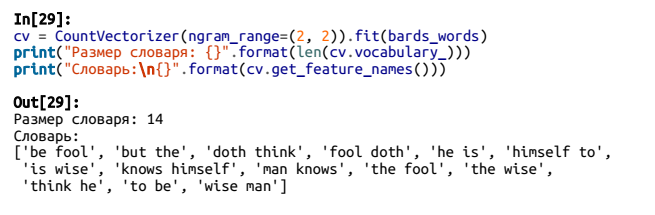
\includegraphics[scale=0.75]{images/lec09-pic29.png}
\end{figure}
\end{frame}

\begin{frame}{Модель <<мешка слов>> для n-грамм}
Использование более длинных последовательностей токенов, как правило, приводит к гораздо большему числу признаков и большей детализации признаков. Нет ни одной биграммы, которая встретилась бы
в обоих строках массива bard\_words:
\begin{figure}[h]
\centering
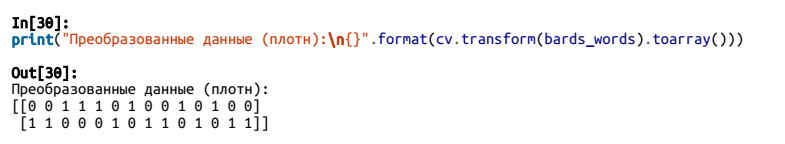
\includegraphics[scale=0.75]{images/lec09-pic30.png}
\end{figure}
\end{frame}

\begin{frame}{Модель <<мешка слов>> для n-грамм}
\begin{itemize}
\item в большинстве прикладных задач минимальное количество токенов должно быть равно единице; \item добавление биграмм помогает в большинстве случаев;
\item включение в анализ более длинных последовательностей, тоже,
вероятно, поможет, но это вызовет взрывной рост количества признаков. 
\end{itemize}
\begin{figure}[h]
\centering
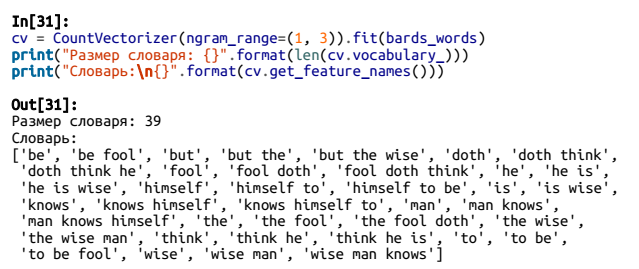
\includegraphics[scale=0.5]{images/lec09-pic31.png}
\end{figure}
\end{frame}

\begin{frame}{Модель <<мешка слов>> для n-грамм для киноотзывов}
Применим TfidfVectorizer к киноотзывам, собранных на сайте IMDb, и найдем оптимальное значение ngram\_range с помощью решетчатого поиска:
\begin{figure}[h]
\centering
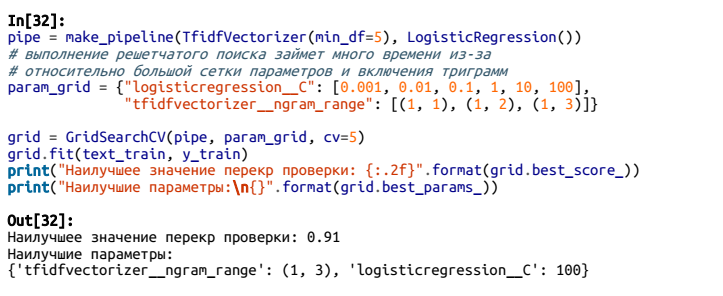
\includegraphics[scale=0.6]{images/lec09-pic32.png}
\end{figure}
Из результатов видно, что мы улучшили качество чуть более чем на один процент, добавив биграммы и триграммы. 
\end{frame}

\begin{frame}{Модель <<мешка слов>> для n-грамм для киноотзывов}
Применим TfidfVectorizer к киноотзывам, собранных на сайте IMDb, и найдем оптимальное значение ngram\_range с помощью решетчатого поиска:
\begin{figure}[h]
\centering
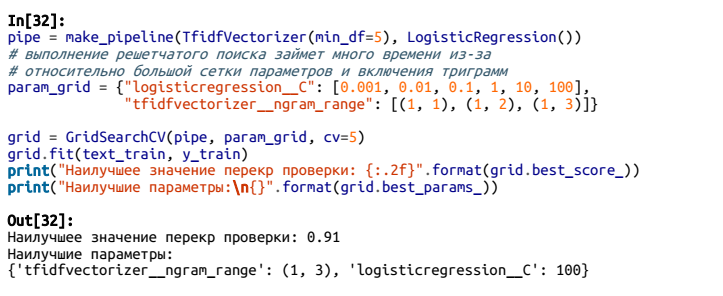
\includegraphics[scale=0.6]{images/lec09-pic32.png}
\end{figure}
Из результатов видно, что мы улучшили качество чуть более чем на один процент, добавив биграммы и триграммы. 
\end{frame}

\begin{frame}{Модель <<мешка слов>> для n-грамм для киноотзывов}
Мы можем представить правильность перекрестной проверки в виде функции параметров
ngram\_range и C, использовав теплокарту:
\begin{figure}[h]
\centering
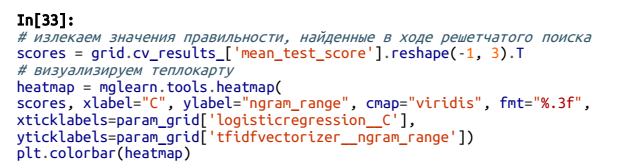
\includegraphics[scale=0.75]{images/lec09-pic33.png}
\end{figure}
На теплокарте видно, что использование биграмм довольно значительно увеличивает качество модели, тогда как добавление триграмм дает очень небольшое преимущество с точки зрения правильности. 
\end{frame}

\begin{frame}{Модель <<мешка слов>> для n-грамм для киноотзывов}
Визуализируем наиболее важные коэффициенты наилучшей модели, которая включает юниграммы, биграммы и триграммы:
\begin{figure}[h]
\centering
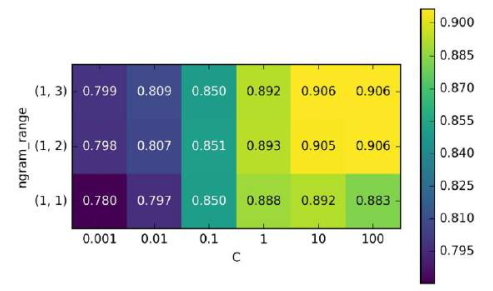
\includegraphics[scale=0.5]{images/lec09-pic34.png}
\end{figure}
\end{frame}

\begin{frame}{Модель <<мешка слов>> для n-грамм для киноотзывов}
Визуализируем наиболее важные коэффициенты наилучшей модели, которая включает юниграммы, биграммы и триграммы:
\begin{figure}[h]
\centering
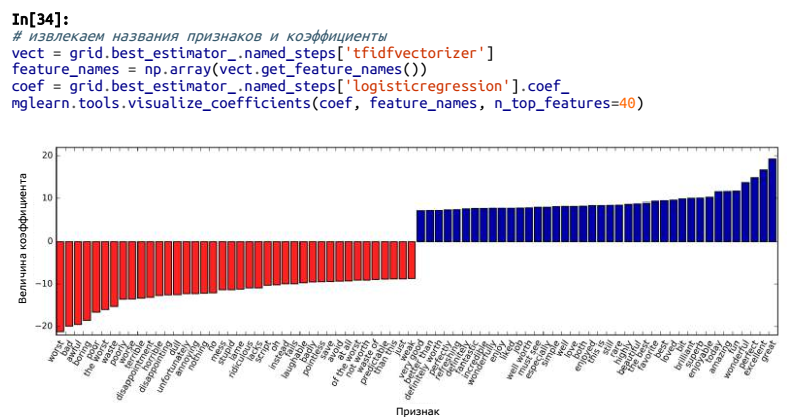
\includegraphics[scale=0.5]{images/lec09-pic35.png}
\end{figure}
У нас появились весьма интересные признаки со словом «worth», которые отсутствовали в юниграммной модели: "not worth" признак указывает на отризательный отзыв, в то время как "definitely worth" и
"worth" свидетельствуют о положительном отзыве. 
\end{frame}

\begin{frame}{Модель <<мешка слов>> для n-грамм для киноотзывов}
Визуализируем только триграммы, чтобы лучше понять, какие признаки являются полезными. 
\begin{figure}[h]
\centering
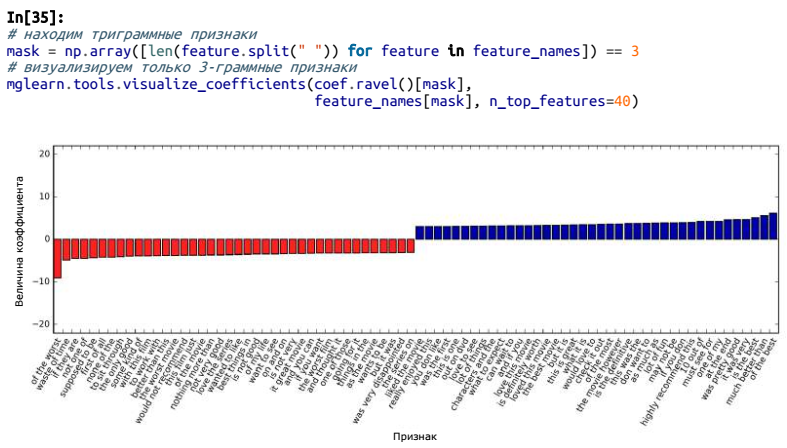
\includegraphics[scale=0.5]{images/lec09-pic36.png}
\end{figure}
Влияние триграммных признаков по сравнению с важностью юниграммных признаков выражено гораздо слабее.
\end{frame}

\end{document}